\documentclass[11pt]{article}
\pdfcompresslevel=0
\pdfobjcompresslevel=0
\usepackage[utf8]{inputenc}
\usepackage[T1]{fontenc}
\usepackage[english]{babel}
\usepackage{
	geometry,
	amsthm,
	amsmath,
	amssymb,
	enumitem,
    microtype,
	setspace,
    xcolor,
    mlmodern,
    % lmodern,
    tikz-cd,
    dsfont,
    float,
}

\geometry{
margin=1.5in % i keep it in 1.5in for the only reason that the title fit in one line
}
% \onehalfspacing
% \setstretch{1.15}    
\theoremstyle{definition}
\newtheorem{prop}{Proposition}
\newtheorem{example}{Example}
\newtheorem{defi}{Definition}
\newtheorem{remark}{Remark}
\raggedbottom
% \setlength{\parindent}{0cm}
\addto\captionsfrench{\renewcommand\proofname{\textbf{\upshape Démonstration.}}}
% \renewcommand{\proofname}{\textbf{Démonstration}}
\color{black!90}
% \renewcommand{\emph}[1]{{\slshape #1}}
% \tikzcdset{arrow style=math font}

\usepackage{hyperref}
\hypersetup{
pdfauthor = {Christian Chávez},
pdfsubject = {Activités de Recherche I - UdeS},
hidelinks,
}

% ----------------------------------------

\newcommand{\R}{\mathbb{R}}
\newcommand{\C}{\mathbb{C}}
\newcommand{\Q}{\mathbb{Q}}
\newcommand{\Z}{\mathbb{Z}}
\newcommand{\red}[1]{\textcolor{red}{#1}}
\renewcommand{\mathbb}[1]{\mathds{#1}}

 


% Title info ---------------------------------------
\title{Computing the interleaving distance between two interval modules}
\author{Christian Chavez} 
\date{}
\begin{document}
\maketitle


I found nowhere the explicit computation of the interleaving distance between
interval modules, tough it is well known that it equals the bottleneck distance.
 

\section{Preliminaries}

Let \(\mathbf{k}\) be an arbitrary field, fixed throughout.
We   denote by  \(\R\)
either the real line or 
the category induced by the poset \((\R,\leq)\).
All functors are covariant.

\subsection{The category of persistence modules}

A \textbf{persistence module} is a functor \(\mathbb{R}\to \mathrm{Vect}(\mathbf{k} )\).

\begin{example}[Important]
Let \(I\subseteq \R\) be an interval.
Define \(\mathbf{k}^I\colon \mathbb{R}\to \mathrm{Vect}(\mathbf{k} )\)
by
\[
t\mapsto \begin{cases}
\mathbf{k} &\text{ if } t\in I\\
0&\text{ else }
\end{cases}
\qquad\text{and}\qquad
r\to s\; \mapsto \begin{cases}
\mathbf{k}\xrightarrow{\mathrm{Id}} \mathbf{k} &\text{ if } r,s\in I\\
0&\text{ else }
\end{cases}
\]
on objects and morphisms, respectively.
We call \(\mathbf{k}^I\) the \textbf{interval module} over \(I\).
\begin{figure}[!h]
\centering
\includegraphics[width=\linewidth]{../assets/media/interval_module.gif} 
\end{figure}

\end{example}

\paragraph{Remark.}
Interval modules are the building blocks of persistence modules.
In fact, one objective of persistence theory is to understand 
persistence modules by decomposing them into interval modules.
However, this is not always possible.
A situation when such a decomposition is   guaranteed is 
when   we work with finite dimentional vector spaces,
that is, if we work over \(\mathrm{vect}(\mathbf{k} )\)
instead of \(\mathrm{Vect}(\mathbf{k} )\).

The   concise definition of persistence module can be expanded to aide 
comprehension.
Let \(V\colon \R\to \mathrm{Vect}(\mathbf{k} )\) be a persistence module.
\begin{itemize} 
\item For each \(t\in \R \) and each arrow \(r\to s\) denote \(V(t)=V_t\) and   \(V(r\to s) = v_s^r\).
\item Since \(V\) is a functor, we have the so-called \textbf{composition law}:
\[
 v_t^s\circ v_s^r = v_t^r\quad\text{ whenever } r\leq s\leq t
\]
and \(V(t\to t) = v_t^t = \mathrm{Id}_{V_t}\).
\end{itemize}
Thus, a persistence module \(V\) is a  family of vector spaces \((V_t)_{t\in \R}\)
together with a family
\((v_t^s \colon V_s\to V_t\mid s\leq t)_{s,t\in\R}\)
of \( \mathbf{k} \)-linear maps 
that satisfy the composition law. 

We got a  set theorical definition from the  categorical one above.
In fact, the  two are equivalent.
We will use the first, but   prefer the notation of the second.

Since persistence modules are functors, we can consider the natural transformations
between them, and since those can be composed (using vertical composition)
we obtain a category.

\begin{defi}
The \textbf{category of persistence modules} is 
\(\mathbf{X} = \mathrm{Fun}(\R, \mathrm{Vect}(\mathbf{k} ))\).
% whose 
% \begin{itemize}
% \item objects are functors \(\mathbb{R}\to \mathrm{Vect}(\mathbf{k} )\), and 
% \item morphisms are natural transformations
% \end{itemize}
%
\end{defi}

Yes, this category is fun.
Concretely,
a morphism of persistence modules \(\alpha\colon U\to V\)
is a family of linear maps 
\((\alpha_r\colon U_r\to V_r)_{r\in \R}\)
such that 
the diagram 
\[
\begin{tikzcd}
U_s \arrow[r, "u_t^s"] \arrow[d, "\alpha_s"'] & U_t \arrow[d, "\alpha_t"] \\
V_s \arrow[r, "v_t^s"]                        & V_t                      
\end{tikzcd}
\]
commutes for all \(s\leq t\).
\subsection{The shift functor}


Let \(U\) be a persistence module.
Define a new persistence module \(U[t]\) by 
\[
% U[t](r)=(U[t])_r = U_{t+r}
% \quad\text{and}\quad 
% U[t](r\to s)=(u[t])_r^s = u_{t+r}^{t+s}
%
U[t](r)  = U_{t+r}
\quad\text{and}\quad 
U[t](r\to s) = u_{t+r}^{t+s}.
\]
We say that \(U[t]\) is a \textbf{shifted module}.

Suppose we've made two shifts of \(U\), say \(U[s]\) and \(U[t]\), where \(s\leq t\).
We might ask ourserlves: what is the relationship between these shifted modules?
Since these are functors, we wonder if there is a canonical natural transformation
\(\alpha\colon U[s]\to U[t]\),
and in fact there is.
To find out, consider any \(p\to q\) and apply both  \(U[s]\) and \(U[t]\) to this arrow.
We get 
$$
U[s](p\to q)\; =\; U_{p+s}\xrightarrow{u_{q+s}^{p+s}} U_{q+s}
$$
and 
$$
U[t](p\to q) \;=\; U_{p+t}\xrightarrow{u_{q+t}^{p+t}} U_{q+t}
$$
% Since \(\alpha=(\alpha_r\colon U[s](r) \to U[t](r))_{r\in \R}\) 
Since \(\alpha=(\alpha_r )_{r\in \R}\) 
is determined by its components,
we need to find the vertical arrows 
that make the square
$$
\begin{tikzcd}
U_{p+s} \arrow[r, "u_{q+s}^{p+s}"] \arrow[d, "\alpha_p"'] & U_{q+s} \arrow[d, "\alpha_q"] \\
U_{p+t} \arrow[r, "u_{q+t}^{p+t}"']                       & U_{q+t}                      
\end{tikzcd}
$$
%
commute. 
Set \(\alpha_p = u_{p+t}^{p+s}\) and \(\alpha_{q}=u_{q+t}^{q+s}\).
Then the composition law give us 
\[
u_{q+t}^{p+t} \circ  u_{p+t}^{p+s} = u_{q+t}^{p+s} = u_{q+t}^{q+s}\circ u_{q+s}^{p+s},
\]
which means the square commutes.
Thus \(\alpha\) is indeed a natural transformation, that we'll denote \(U[s\to t]\).
To sum up, we have the following natural transformation 
% $$
% \begin{tikzcd}
%   \R
%     \arrow[r, bend left=35,  "U[s]" name=Us,  below]
%     \arrow[r, bend right=35, "U[t]"' name=Ut]
%   & \mathrm{Vect}(\mathbf{k})
%     \arrow[Rightarrow, from=Us, to=Ut, "\alpha"]
% \end{tikzcd}
% $$


% \[
% \begin{tikzcd}[column sep=huge]
% \R  \arrow[bend left=50]{r}[name=0,anchor=center, inner sep=0, "U[s]"]
%   \arrow[bend right=50]{r}[name=1,label=below:$\scriptstyle U$] &
% \mathrm{Vect}(\mathbf{k} )
%   \arrow[shorten <=10pt,shorten >=10pt,Rightarrow,to path={(0) -- node[label=right:$\det$] {} (1)}]
% \end{tikzcd}
% \]
% where 
$$
U[s\to t] = \left( u_{t+r}^{s+r} \right)_{r\in \R}.
$$
On the other hand, note that 
$$
U[t][t'] = U[t+t']
$$
for any \(t,t'\in R\).

% Note that \([t]\) is a functor \(X\to X\) . THIS IS FALSE.

\begin{figure}[h]
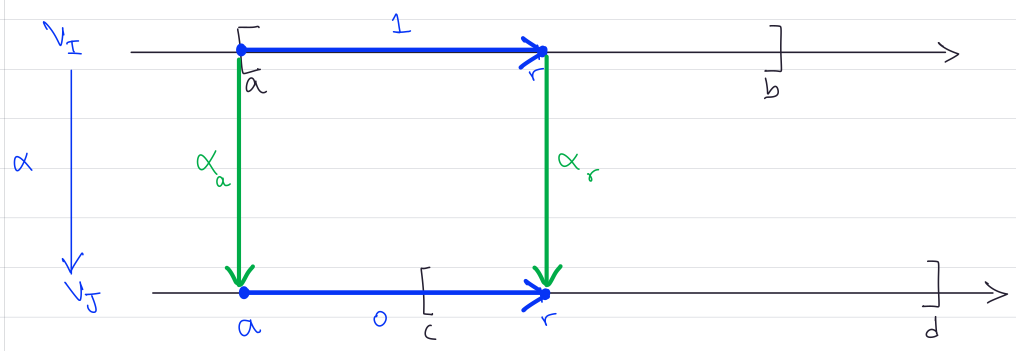
\includegraphics[width=\linewidth]{../assets/media/nt.png}
\end{figure}

The functor \(T = [\,\cdot\,]\colon \R\to \mathrm{End}(X)\) 
is defined as follows
\begin{itemize}
\item Objects: for each \(t\in \R\) we have a functor  \(T(t) \colon X\to X\) denoted  \(T_t\), which is defined by \(T_t( U) = U[t]\) on objects \(U\in X\), and by \(T_t(\alpha) = (\alpha_{r+t})_{r\in \R}\) on morphisms \(\alpha=(\alpha_r)_{r\in \R}\). (Equivalently, we can define \(T_t(\alpha) = \alpha \star [t]\))
\item Morphisms: for each \(r\to s\), define    a natural transformation $T(r\to s)\colon T_r\to T_s$ by
$$
T(r\to s)\colon T_r\to T_s = \left( U[r\to s] \right)_{U\in X}
$$
\end{itemize}
 
\subsection{The interleaving distance between persistence modules}

Let \(U\) and \(V\) be persistence modules.
A \(t\)-\textbf{interleaving} of \(U\) and \(V\) is a pair of morphisms 
\((\phi, \psi )\)
that make the   diagrams 
\[
\begin{tikzcd}
U \arrow[rd, "\phi"'] \arrow[rr, "\mathbb{1}^{2t}_U"] &                                 & {U[2t]} & V \arrow[rd, "\psi"'] \arrow[rr, "\mathbb{1}^{2t}_V"] &                                 & {V[2t]} \\
                                                      & {V[t]} \arrow[ru, "{\psi[t]}"'] &         &                                                       & {U[t]} \arrow[ru, "{\phi[t]}"'] &        
\end{tikzcd}
\]
commute.
If such a pair exists, we say that \(U\) and \(V\) are \(t\)-interleaved.



\begin{defi}
The  interleaving distance 
between two interval modules is
\[
d_T (U, V)=\inf \left\{t\geq 0 \mid \text { there exists a } t\text {-interleaving of } U \text { and } V\right\}.
\]
\end{defi} 
This is the smallest shift we'd need to do for...

\section{The computation}

We'll do the computation for the case of closed intervals.
Let \(I=[a,b]\) and \(J=[c,d]\).
Denote by  $\mathcal{I}=\mathbf{k}^I$ and $\mathcal{J}=\mathbf{k}^J$   the corresponding 
interval modules.

Our strategy is  to find some apropriate bounds for $d_T (U, V)$.
Befor going into the search for the pair of morphisms 
that would make the triangles above commute,
we need to know how are the morphisms between interval modules,
because then we can characterize the morphisms between
shifted interval modules.



\subsection{Bound above}


\subsection{Bound below}

\end{document}